\documentclass[11pt]{article}
\usepackage[margin=1in]{geometry}
\usepackage{amsmath,amssymb}
\usepackage{booktabs}
\usepackage{xcolor}
\usepackage{graphicx}
\usepackage{parskip}
\usepackage{listings}
\usepackage{tikz}
\usetikzlibrary{positioning,arrows.meta,fit,backgrounds,calc,shapes.geometric}
\usepackage[colorlinks=true,linkcolor=blue,urlcolor=blue,citecolor=blue]{hyperref}

\definecolor{cset}{RGB}{31,119,180}
\definecolor{cfield}{RGB}{44,160,44}
\definecolor{cop}{RGB}{214,39,40}
\definecolor{cgray}{RGB}{120,120,120}
\definecolor{cwarn}{RGB}{181,133,47}

\newcommand{\code}[1]{\texttt{#1}}

\title{\textbf{Plexus Discovery}\\[3pt]
\large Searching for mechanisms instead of tuning parameters}
\author{Janelia Research Campus}
\date{\today}

\begin{document}
\maketitle

\begin{abstract}
\noindent
This note is a companion to \emph{Plexus: A blueprint for differentiable tissue}. That paper
describes a language for writing biological mechanisms down. This note describes what we do
with the language: an automated loop that \emph{searches} for the mechanism behind an observed
morphology, rather than assuming one and tuning its parameters.

It is written to be read before the loop is switched on for a long run. So it is deliberately
part description and part criticism. Section~\ref{sec:wrong} lists what is currently wrong with
our implementation, including two mistakes that already produced a result we believed for
several days and that was not real. Section~\ref{sec:foundation} states what we fix first.
No machine-learning or physics background is assumed.
\end{abstract}

\section{The question this note answers}

A microscope movie shows an embryonic gland turning into a branched tree, or a sheet of cells
folding into a tube. We would like to know \emph{why}: which cellular behaviours, acting
together, produce that shape.

The usual approach is to write a computer simulation that we believe captures the biology, then
adjust its numbers until the simulation resembles the movie. This works well when we already
know which biology matters. In development we usually do not. Many mechanisms have been
proposed for branching alone: chemical pre-patterns, differential stickiness between cells,
matrix deposited at the surface, mechanical buckling. Each has a paper. Few have been compared
head to head, and almost none have been tested in combination --- yet a combination is the
likeliest explanation of a shape that no single mechanism fully reproduces.

So the honest question is not \emph{what are the parameters?} It is \emph{what is the model?}

\section{A mechanism, written down}

Plexus writes a biological model as a small number of named \emph{operators} wired together.
An operator is one biological verb: cells stick together, a signal diffuses, a cell divides,
tissue grows where a signal is strong. Each operator says what it acts on and what it changes.
A model is then not a monolithic program but a short recipe --- which verbs are present, and
what feeds what.

\begin{center}
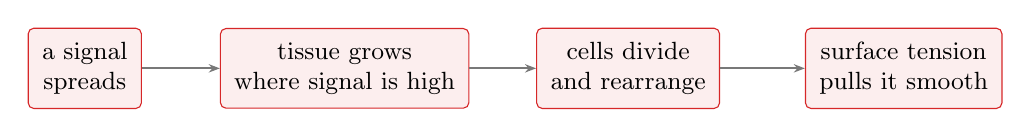
\begin{tikzpicture}[
  op/.style={rounded corners=2pt, draw=cop, fill=cop!8, align=center, inner sep=5pt,
             minimum height=0.95cm, font=\small},
  ar/.style={-{Stealth[length=4pt]}, draw=cgray, line width=0.8pt}]
\node[op] (rd)   at (0,0)    {a signal\\spreads};
\node[op] (grow) at (3.3,0)  {tissue grows\\where signal is high};
\node[op] (div)  at (6.9,0)  {cells divide\\and rearrange};
\node[op] (mech) at (10.4,0) {surface tension\\pulls it smooth};
\draw[ar] (rd) -- (grow);
\draw[ar] (grow) -- (div);
\draw[ar] (div) -- (mech);
\end{tikzpicture}
\end{center}
{\small\emph{A mechanism as a recipe of operators. Changing the wiring --- routing the signal to
control division instead of growth --- is a different mechanism, not a different parameter.}}

This matters for one reason. Because a model is a recipe, we can \emph{edit} it: add a verb,
remove a verb, or re-route what feeds what. That turns ``which model?'' into something a
computer can search, in the same way that ``which parameters?'' already is.

\section{Why parameter tuning cannot find a mechanism}

We learned this the expensive way, and it is worth stating plainly because it is the reason the
loop exists.

We spent roughly thirty rounds trying to reproduce a published result: a sheet of cells that
grows a tube. Each round adjusted numbers --- how fast cells grow, how strong the signal is, how
stiff the tissue is. Each round failed in a slightly different costume. Either the activated
patch ballooned into a bulge, or the whole shell inflated uniformly and stayed flat. There was
no setting in between.

The conclusion, once we finally drew it, was that the missing ingredient was not a number. Our
representation could not hold a tube: it had no way to express a narrow neck that stays narrow
while its tip advances. That is a property of the \emph{recipe}, not of its settings. And a
search over settings cannot escape a limitation of the recipe --- not with more compute, not
with more rounds. Every round was locally sensible and collectively doomed.

This is the trap the loop is built to avoid, and the discipline it enforces is simple: a change
of numbers is never allowed to count as a new hypothesis.

\section{The loop}

We separate three questions that a single optimisation silently mixes together.

\begin{center}
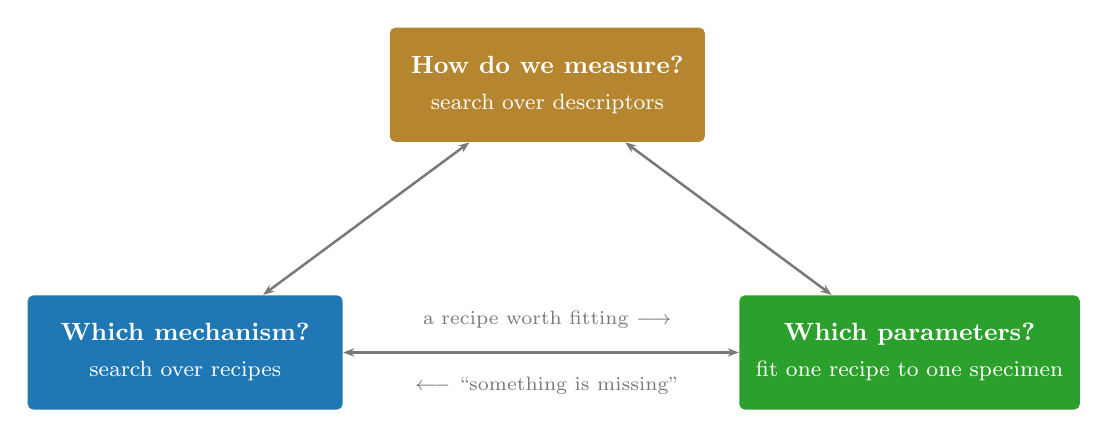
\begin{tikzpicture}[
  box/.style={rounded corners=2pt, align=center, text=white, inner sep=6pt,
              minimum width=4.0cm, minimum height=1.45cm, font=\small},
  sig/.style={font=\scriptsize, text=cgray, align=center},
  edge/.style={{Stealth[length=4pt]}-{Stealth[length=4pt]}, line width=0.9pt, draw=cgray}]
\node[box, fill=cset]   (I)   at (-4.6,0) {\textbf{Which mechanism?}\\[2pt]\footnotesize search over recipes};
\node[box, fill=cfield] (II)  at ( 4.6,0) {\textbf{Which parameters?}\\[2pt]\footnotesize fit one recipe to one specimen};
\node[box, fill=cwarn]  (III) at ( 0,3.4) {\textbf{How do we measure?}\\[2pt]\footnotesize search over descriptors};
\draw[edge] (I) -- (II);
\draw[edge] (I) -- (III);
\draw[edge] (II) -- (III);
\node[sig] at (0,0.42) {a recipe worth fitting $\longrightarrow$};
\node[sig] at (0,-0.42) {$\longleftarrow$ ``something is missing''};
\end{tikzpicture}
\end{center}

\textbf{Which mechanism?} The computer starts from a bare recipe and edits it one verb at a
time. A recipe is credited only if the shape appears across a \emph{range} of settings and
several random seeds --- not at one lucky setting. The output is not a best-fitting simulation;
it is knowledge of the form ``growth plus surface tension plus a cleft-forming step reproduces
this; adhesion alone provably cannot.''

\textbf{Which parameters?} Only once a recipe has earned trust do we fit it to a particular
specimen. Because every operator is differentiable, this is fast and exact. Importantly, the fit
returns not just the best numbers but the \emph{leftover disagreement}. A disagreement that will
not go away, no matter the numbers, is evidence that a verb is missing --- and it is handed back
to the first question rather than papered over.

\textbf{How do we measure?} A simulation is compared to data only through some measurement. Our
measurements are hypotheses too, and a bad one is dangerous in a specific way: it can call a
wrong simulation right. This is not hypothetical. We had a run whose numerical scores were all
acceptable while the picture showed a lumpy blob rather than tubes; the scores measured how far
things stuck out, and a blob sticks out. We only caught it by inventing a new measurement (how
tightly the signal stays confined). So the loop also searches for better observables, and a new
measurement is admitted only if it agrees with expert-annotated ground truth, separates
mechanisms we already know differ, and is insensitive to irrelevant details like random seed.

The three run as a ladder, not as three simultaneous searches: one is exploratory at a time and
the other two are frozen as anchors. The parameter fit is earned last, never first.

\section{What the loop has already done}

The loop is not a proposal. A version of it has run on embryonic salivary gland branching, using
real imaging data, and produced the following sequence without human steering.

\begin{enumerate}\itemsep2pt
\item A representation of the tissue as $\sim$600 individually migrating cells was shown to be
\emph{incapable} of the phenotype --- it can only break into fragments, whereas the real gland
stays one connected mass. None of that search's 28 apparent winners survived a corrected
readout. This is a failure of representation, not of fitting, and no amount of tuning addresses it.
\item Switching to a dense representation, in which the tissue is connected by construction, made
the search possible.
\item The search then found a recipe --- growth, surface tension, and a surface-driven cleft ---
that reproduces branching robustly, and recorded genuine impossibility results along the way
(``no growth: never develops''; ``no cleft: grows into a blob but cannot subdivide'').
\item Two rival recipes remained that the measurement of the day could not tell apart. That
failure justified inventing a better measurement, which then \emph{changed the conclusion} ---
and did so by re-scoring simulations already in the archive, without re-running any of them.
\end{enumerate}

Point 4 is the one we care about most. A new way of looking at the data revised a mechanistic
conclusion. That is measurement science, and it is what the loop is for.

\section{What is currently wrong with it}
\label{sec:wrong}

This is the important section. The loop is about to run for weeks, and its output will be
scientific claims --- including claims that something is \emph{impossible}. A wrong impossibility
claim is worse than no claim at all, because it closes a question that should stay open. So we
audited our own implementation adversarially. Six problems, in order of how much damage they do.

\paragraph{1. Two of our operators kept a private clock.}
Several operators were written to act every second or third step, and the simulation engine
\emph{also} spaces them out. The two schedules multiplied. An operator marked ``every 2 steps''
actually fired every 4. Cell division across every run we have archived therefore happened at a
fraction of the advertised rate. Nothing crashed; the numbers were simply not the numbers we
thought. \emph{Fixed: the engine owns the clock; the private ones are deleted, and the affected
baselines are re-measured and re-recorded.}

\paragraph{2. Adding a signalling step silently changed the clock.}
Our run script chose the simulation time-step based on \emph{which operators were present}:
recipes containing a chemical signal ran with a time-step fifty times smaller. This is
catastrophic for a mechanism search, because the loop's single most important edit is adding or
removing the signalling step --- and under this rule that edit also changed the ratio between
chemical and mechanical time. Every conclusion about whether signalling matters would have been
confounded. \emph{Fixed: one time-step for the whole search, set explicitly; stability needs are
handled inside the operator that has them.}

\paragraph{3. A silent mismatch produced a result we believed for days.}
Positions and connectivity were recorded on different schedules. When they drifted out of step,
the analysis paired each cell's position with a \emph{different moment's} connectivity. The
result was a spectacular artefact: cells appeared inverted and hollow, and we spent days
diagnosing ``global buckling'' that never happened. Every proposed physical cure failed, which
in hindsight was the clue. \emph{Fixed: the two must now be the same length, and this is asserted
rather than quietly patched --- the original code silently clamped the mismatch away.}

\paragraph{4. An operator that does nothing still returns numbers.}
Some operators only work if another ran first --- a signal cannot spread before neighbours are
computed. If the prerequisite is missing, the operator does nothing, and the simulation still
finishes and still produces a score. Under hand-written recipes this was harmless, because a
human wrote the prerequisites in. Under an automatic search it is the most dangerous bug
possible: the loop would record ``this mechanism cannot make tubes'' when in truth the mechanism
never ran. \emph{Fixed: prerequisites are now declared and checked, and every operator reports
whether it actually did anything; a run in which a scheduled operator never acted is an error,
not a result.}

\paragraph{5. Some operators advertised capabilities they do not have.}
One is labelled as differentiable but internally discards gradients. Another claims to work in
three dimensions while its validity check is two-dimensional geometry, so its verdict in 3D was
arbitrary. Labels that lie are worse than absent labels, because the search trusts them.
\emph{Fixed: labels corrected, and a check now certifies them mechanically.}

\paragraph{6. Our measurements can pass while the picture is wrong.}
Discussed above: a lumpy blob scored acceptably on every number we had. This is not a bug to fix
once; it is a permanent hazard of automated science, and the only defence is to keep looking at
the pictures and to invent a new measurement whenever the eye and the number disagree.
\emph{Mitigation: before the search is trusted, the measurement suite must first correctly
separate a set of already-archived runs that we have labelled by eye. If the instrument cannot
reproduce our own judgement on known cases, it is not ready to judge unknown ones.}

We also record one deliberate difference from comparable automated-discovery systems in the
literature. Those systems rank competing hypotheses by having a language model debate them,
because their experiments are slow and expensive (they are wet-lab experiments). Our experiments
are simulations that take seconds. We therefore rank by \emph{measuring}, and use the language
model only to propose recipes and to describe results in words. Where the ground truth is
available, an opinion about it is a step backwards.

\section{The foundation we build first}
\label{sec:foundation}

\subsection{Do the operators belong in the core library?}

The tissue-mechanics and reaction-diffusion operators were developed in a prototype folder. The
natural instinct before a long campaign is to promote them into the core library and make them
fully conformant. We tested that instinct and it did not survive contact with the facts.

Loading the prototype adds its operators to \emph{the same registry} the core library uses ---
52 operators become 79 --- and they are validated, scheduled, and executed by exactly the same
machinery. Promotion, in other words, moves files. It adds no capability, and it fixes none of
the six problems above. Meanwhile it is not a small job: the core library has no concept of a
mesh whose cell count grows during a run, so a faithful promotion is a substantial engine
project, and it would consume the time the campaign itself needs.

So we separate two things that were tangled together: \emph{where an operator lives} and
\emph{whether it is correct and honestly labelled}. The second is what actually protects the
science, and it can be had now. Concretely we (i) make the mesh a proper object rather than an
untyped bag of arrays, with the geometric invariants as enforced methods; (ii) fix the six
problems above; (iii) declare the full contract on every operator the search will use; and (iv)
extend the conformance checker so a prototype-resident operator can be \emph{certified} without
being moved. Promotion into the core library then happens later, for the operators the campaign
demonstrates are worth keeping --- which is the right criterion for what belongs in a shared
library anyway.

\subsection{Making the mesh honest}

The tissue is represented as a mesh: cells are faces, and the corners they share are the
quantities the physics actually moves. This was stored as an untyped collection of arrays,
which is how several of the problems above became possible.

It is now an object with its invariants built in, and one of those invariants deserves a note
because it caught a real error. A face must not be self-intersecting --- a bow-tie. We had
checked validity by computing area and requiring it to be positive. A bow-tie has positive area.
So the check passed, the mesh was tangled, and a quantitative result about cell rearrangement
was wrong; it was caught by looking at a rendered movie, not by any number. The lesson
generalises beyond meshes: \emph{a numerical invariant is not the same as the geometric one},
and a picture is often the sharper test.

\subsection{How we will know it works}

One command runs a ladder of checks, each reported separately. The ladder matters more than any
single check, because each level catches a class of error the others cannot see.

\begin{center}
\small
\begin{tabular}{@{}lll@{}}
\toprule
\textbf{Level} & \textbf{What it checks} & \textbf{The error class it catches} \\
\midrule
Contract      & every operator declares what it is and does & labels that lie \\
Unit          & each operator reproduces its previous output & the refactor changed physics \\
Trajectory    & a whole run reproduces its recorded history & schedule or ordering changed \\
Invariants    & closed surface, no tangled or bow-tie faces & silent geometric corruption \\
Recording     & positions and connectivity are the same length & the phantom-result bug \\
Metrics       & scores match archived values & the analysis path drifted \\
Gradients     & derivatives flow and are finite & parameter fitting will fail later \\
Coverage      & every operator is exercised by some test & untested code presumed working \\
Description   & a vision model's caption matches expectation & the numbers pass, the picture is wrong \\
\bottomrule
\end{tabular}
\end{center}

The last row is unusual and worth explaining. Every simulation we generate is automatically
described in words by a vision model watching the movie. We had adopted this for documentation.
It doubles as a test: if a run that should be ``a sphere growing narrow tubes'' is described as
``a scattered cloud of red patches'', no numerical score caught it but the caption did. It is a
cheap, independent check against exactly the failure mode of section~\ref{sec:wrong}, item~6.

\section{What will count as a result}

The campaign runs for weeks and produces a ledger rather than a single best simulation. Every
claim in it is sorted into one of four kinds:

\begin{center}
\small
\begin{tabular}{@{}ll@{}}
\toprule
\textbf{Established} & the operator is necessary, sufficient, and works across a range of settings \\
\textbf{Refuted} & contradicted across independent repeats \\
\textbf{Structural limitation} & this recipe \emph{cannot} produce the phenotype at all \\
\textbf{Open} & not yet decided \\
\bottomrule
\end{tabular}
\end{center}

A mechanism is promoted to \emph{Established} only if it answers the three questions a biology
paper would ask: remove it --- does the shape collapse? Is a minimal recipe containing it
sufficient? Does it survive across repeats and a range of settings?

We want to be explicit that \emph{Structural limitation} is a real result and not a failure to
report. ``This family of recipes cannot make a tube'' is reusable knowledge that saves the next
person the thirty rounds it cost us. It is also, precisely because it is a strong claim, the
result most easily faked by the bugs in section~\ref{sec:wrong} --- which is why the foundation
work comes first.

\section{Status}

The loop has run on gland branching. The mechanics and signalling operators for the second
system --- a growing cell sheet that should form tubes --- exist and are being hardened as
described above. The campaign starts once the measurement suite has demonstrably reproduced our
own judgement on runs we have already labelled by eye.

That gate is the point of this note. The system is now capable of running unattended for a long
time and producing confident, well-formatted, entirely wrong conclusions. The defence is not
more compute. It is a small number of checks that fail loudly, an archive that keeps the raw
evidence separate from its interpretation, and the willingness to keep looking at the pictures.

\end{document}
